%===================================== CHAP 2 =================================

\chapter{Modeling neurons}

Before applying statistical tools, it is necessary to define a model that captures the significant features of an actual neural network. The aim of this chapter is to describe the relevant concepts from neuroscience, build a modeling framework that fits to those concepts and to motivate a practical understanding. Section \ref{structure_nn} gives a brief description of signaling and connectivity in neural networks, and the hallmarks for AD in the brain. For the first part the main source used is the book \textit{Neuroscience} \cite{Purves} and for the second part the content is based on sources \cite{Gomez,Witter:2011}. Section \ref{Lab} provides an outline of the lab experiments that produces the data. The information is based on the description of the lab set up in Katrine's master thesis. This is the same lab set up as will be used for this project. In section \ref{set_up} the  framework of the mathematical model is defined with reference to the concepts introduced in the section before. This framework is inspired by the model in Linderman 2016.  

%En av de som Katrine sendte
%http://www.scholarpedia.org/article/Entorhinal_cortex
%https://en.wikipedia.org/wiki/Entorhinal_cortex


\subsection{Related neurology}
\label{structure_nn}

\textsc{Neuron and connections}\\
The brain comprise a complex network of neurons that work together by transmitting signals to each other. The basic unit, the neuron, 
 consists of a cell body (soma), an axon and dendrites. Figure \ref{neuron} shows an illustration of a neuron.
\begin{figure}[h]
    \caption{}
    \label{neuron}
    \centering
    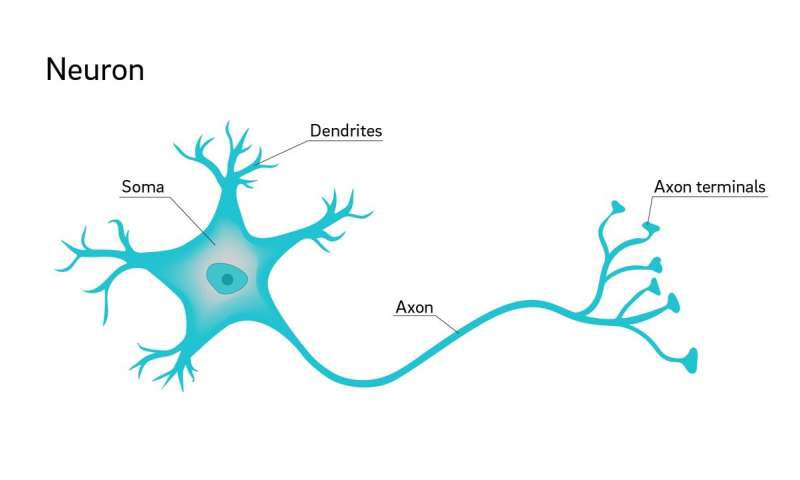
\includegraphics[scale=0.3]{Neuron.jpeg}
\end{figure} 

Neurons can transmit electrical signals to each other through a connection of the axon of one neuron with the dendrite of another. The sending and the receiving neuron are referred to as the "presynaptic neuron" and the "postsynaptic neuron", respectively. Such a connection between two neurons is called a synapse, and is in practice a short gap where chemical units, called neurotransmitters, is allowed to flow from the axon to the dendrite. 

This signaling happens in response to something called an action potential in the presynaptic neuron. When a neuron is at rest, there is a constant potential difference between the inside and the outside of the neuron's cell membrane. An action potential is a rapid increase in this membrane potential, caused by ion flows through channels in the membrane. This action potential then propagates along the axon until it reaches the synapse, and ends up as an electrical signal to the connected neuron. In order for the action potential to occur, the potential difference must reach a certain threshold value. If this threshold is reached, the action potential will take place no matter what. In other words there is an all-or-non property, and if it first takes place the action potential will always have the same strength. This phenomenon is illustrated in figure \ref{AP}.

\begin{figure}[h]
\caption{}
\label{AP}
\begin{subfigure}
\centering
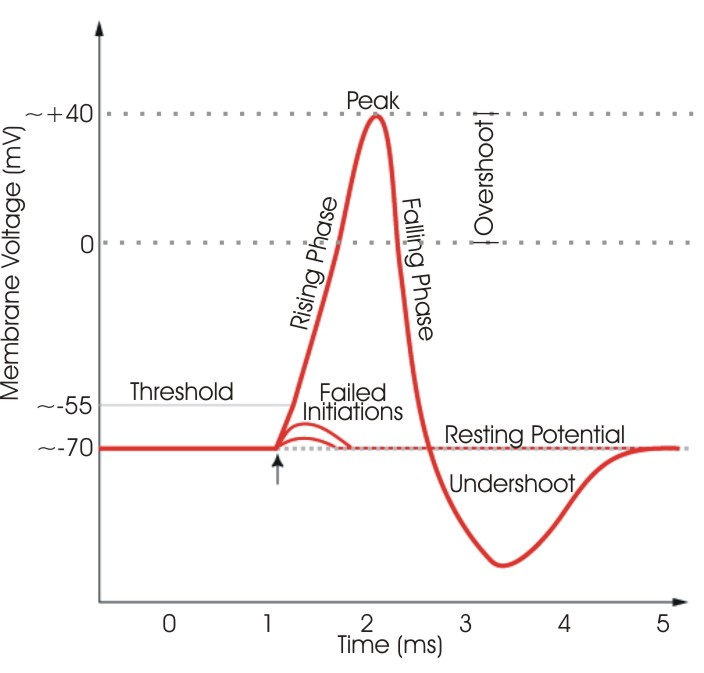
\includegraphics[scale=0.7]{AP.jpg}
\end{subfigure}
\begin{subfigure}
\centering
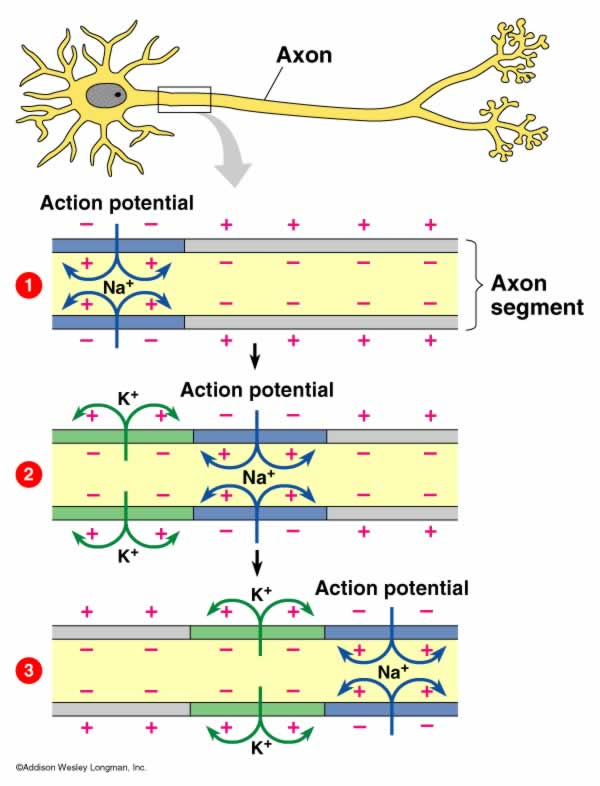
\includegraphics[scale=0.21]{Axjk4.jpg}
\end{subfigure}
\end{figure} 

The developing of an action potential happens in response of some stimuli. This can be external stimuli from some sense, for example a ray of light that hits the eye. Also, action potentials can develop after the receiving of an electrical signal from another neuron. When a signal increase the likelihood of an action potential to also arise in the postsynaptic neuron, this is referred to as an excitatory signal. This enables the possibility for a signal to propagate through the network, and eventually end up for example in a muscle and cause a contraction. On the contrary there are also signals that decrease the chance that the postsynaptic neuron will fire. These are called inhibitory signals.

The  strength of these neural connections are not fixed, but can change over time. Strength of synapses refer to the probability that the postsynaptic neuron will be affected by the signal. A frequent activation of a synapse can strengthen the synaptic connection. This phenomenon is called "long-term potentiation (LTP) of a synapse. Other times activation of a synapse can weaken the connection over time, known as "long-term depression". These changes of connections are referred to as synaptic plasticity, and is the mechanism that gives rise to learning and memory. \\

\textsc{Entorhinal cortex and Alzheimer's disease}

\begin{itemize}
    \item More on this section
    \item Say something about what is known today and what is not. Status of research
    \item Make connection to the work I am going to do. Why do we think that its an idea to invesigate the learning rule in the context of Alzheimer's research
\end{itemize}
%The human brain is very good at forgetting. The hippocampus is a structure in the brain that has been associated with various memory functions

The data basis for this project are lab recordings on mice brains with and without AD. These recordings are done on a part of the brain called he entorhinal cortex. This part is used, since the entorhical cortex is where the earliest indications for AD can be seen. Figure \ref{EC} shows where in the brain the entorhinal cortex is located. 


\begin{figure}[h]
    \caption{}
    \label{EC}
    \centering
    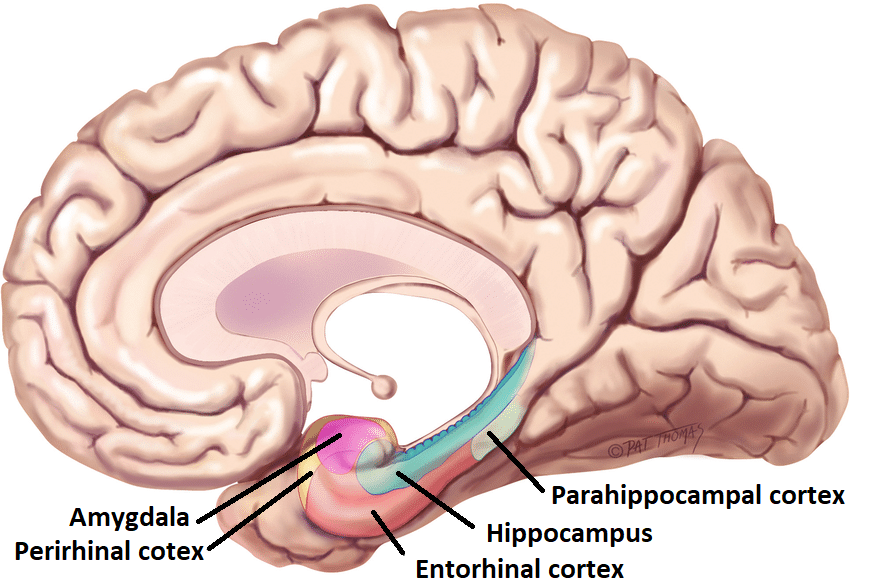
\includegraphics[scale=0.35]{Entorhinal_cortex.png}
    \label{brain}
\end{figure} 

The entorhinal cortex is found in the medial temporal lobe and functions as a gateway between the neocortex and the hippocampus. It is a part of the hippocampal memory system (Witter 2011), and is associated with declarative memory and learning. It is commonly subdivided into six layers, I-VI. It seems like the cells in layer II of the entorhinal cortex are affected in the initial stages of the AD. Characteristic to brains with Alzheimer's is the accumulation of some protein types called amyloid plaques and neurofirbillary tangles, and neuronal loss. 

During the course of Alzheimer's disease there are happening significant changes in the brain. Figure \ref{brain1} illustrates how a brain can look like after having AD for many years.


\begin{figure}[h]
    \label{brain1}
    \centering
    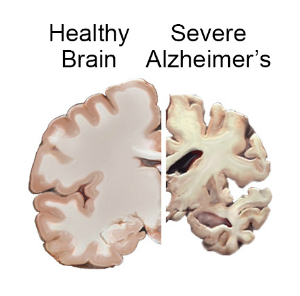
\includegraphics[scale=0.5]{brain_slices_alzheimers_0.jpg}

\end{figure} 


%The entorhinal cortex (EC) is an area of the brain located in the medial temporal lobe and functions as a hub in a widespread network for memory, navigation and the perception of time.[1] The EC is the main interface between the hippocampus and neocortex.  The entorhinal cortex (EC), in particular (Wikipedia)
%the layer II of the domains located towards the collateral/rhinal fissure, contains neurons that are
%among the very first to undergo pathological alterations associated with the disease. Specifically,
%neurons in this domain develop the initial cortical tau pathology, while layer II is also known to
%exhibit severe neuronal loss already during the pre-clinical stages of AD. Furthermore, layer IIneurons are also subject to early accumulation of intracellular Aβ. In order to help enable the study
%of these early neuronal pathologies the work in this thesis was aimed at developing a platform for
%studying the LEC layer II neuronal population in vitro. (Katrines master)

\subsection{Lab recordings}

\label{Lab}\\
The data to be used are recordings from mouse brains with and without Alzheimer's. The ?? are currently in a process of developing techniques to keep the neuronal networks alive long enough for the Alzheimer's disease to develop properly??. However, similar experiments have been performed the last years, and the main techniques are the same. 
\begin{itemize}
    \item Several mice some with and some without Alzheimers. Genetically manipulated? 
    \item Brains extracted, slices from Layer 2 taken out. Kept in dishes
    \item Microelectrode arrays. Equally spaced electrodes that can detect action potentials of single neurons
    
\end{itemize}

Each electrode records the electric potential for one neuron over a time interval.  When a neuron undergoes an action potential, this will appear as a peak in these recordings. It is the time points of these action potentials that are of interest, and not the voltage value itself. Let's label the N recorded neurons with numbers $1,2,...,N$. Then, the gathered data is sequences of time points for the action potentials for each neuron
\begin{equation}
    \{\{ap_i\}\}_{i=1}^{N} = \{ap_{i1}, ap_{i2}, ...\}_{i=1}^{N} \quad ap_{ix} \in [0,T]
\end{equation}

where $ap_{ix}$ is the recorded time for the x'th action potential for neuron $i$, and $ap_{ix-1} < ap_{ix}$. Such a sequence of time stamps for neuron firing is called a spike train. (Illustration of spike trains).\\



\subsection{Model setup}
\label{set_up}

For the later calculations it is practical to represent the spike data in another format. Define

\begin{equation}
    t \in \{t_1, t_2, ..., t_n\} 
\end{equation}

 where $\{t_1, t_2, ..., t_n\}$ is \ a sequence of equally spaced time steps in [0,T], where $t_{k}-t_{k-1} = t_1$. Also let $s_{i,t} \in \{0,1\}$ be a variable taking value 1 if neuron $i$ spikes in the time bin $(t_{k-1}, t_{k})$, and 0 otherwise. To keep as much information as possible, it is preferable to set the time intervals so small that there is very low probability that the neuron will spike more than once in the intervals. Then, at time $t$ we have a collection of $N$ sequences

\begin{equation}
    S_{t} = \{\{s_{i,t_1}, ,...,s_{i,t-1},s_{it}\}\}_{i=0}^{N} \quad s_{i,t_k} \in {0,1}
\end{equation}

This is illustrated in the following figure, where the top array is a spike train, and the bottom array is the corresponding binary values for the time bins

\begin{figure}[h]
    \centering
    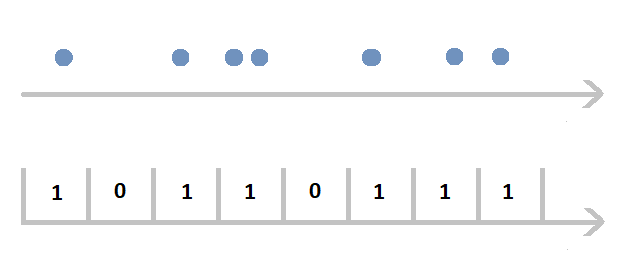
\includegraphics[scale=0.7]{Sp_t.png}
\end{figure} 

The neurons are assumed to be connected in a network. These connections can be represented by a $N \times N$ matrix, $W$, where each element $w_{ij}=w_{ij}$ is a weight corresponding to the strength of the connection between neuron $i$ and neuron $j$. A positive value for $w_{ij}$ corresponds to an excitatory synaptic connection, whereas a negative weight represents an inhibitory. A weight with value zero, means that there is no connection. 
Typically these weights are considered as fixed. However, as the aim is here to study the synaptic plasticity, the weights are let to vary with time. Thus, there is a weight matrix for every time point, $\{W_t\}_{t=0}^{T}$. For a network consisting of three neurons, the weight matrix at time $t$ will look like

\begin{equation*}
W_t = 
\begin{pmatrix}
w_{11,t} & w_{12,t} & w_{13,t}\\
w_{21,t} & w_{22,t} & w_{23,t}\\
w_{31,t} & w_{32,t} & w_{33,t}\\
\end{pmatrix} 
\end{equation*}
\\

\textsc{Learning rules}\\
The way in which the weights are changing is expected to follow some rules, called learning rules. The time development of the weights can be represented by

\begin{equation}
    W_{t+1} = W_t + l(W_t, S_{\leq t}) + \epsilon
\end{equation}

where $l$ is a learning rule depending on the current weights and the spike history. Experimental research have discovered some typical learning rules. One that is famous and quite simple is the spike-timing dependent plasticity (STDP). %https://www.nature.com/articles/nn0900_919 
In this rule the weight between two neurons are updated according to the spike history of those two neurons only. There are other rules where a weight can be dependent on the spike history of the whole network. In the STDP rule the weight $w_{ij}$, going from neuron $i$ to neuron $j$, is increased whenever neuron $j$ spikes shortly after neuron $i$, and decreased if neuron $i$ spikes shortly after neuron $j$. The canonical STDP rule looks like (Linderman dissertation 2016)

\begin{equation}
    \begin{split}
    l(w_{ij}(t), S_{\leq t}) = l_+(S_{<t}, A_+,\tau_+) - l_-(S_{<t}, A_-,\tau_-)\\ 
    l_+(S_{\leq t}, A_+,\tau_+) = s_j(t) \sum_{t'=0}^{t} s_i(t') A_+ e^{(t-t')/\tau_+}\\ 
    l_-(S_{\leq t}, A_-,\tau_-) = s_i(t) \sum_{t'=0}^{t} s_j(t') A_- e^{(t-t')/\tau_-}
    \end{split}
\end{equation}

The parameters $\tau_+$ and $\tau_-$ affects the rage of time intervals in which the spiking contributes to the weight updates. Decreasing the $\tau$ value corresponds to shrinking the window for where spiking has significant impact on the plasticity. According to \cite{Song} experiments have shown that the value for $\tau_+$ is in the order of ten milliseconds. Some experiments suggest a value for $\tau_-$ of the same size, while other suggests a value somewhat larger. The parameters $A_+$ and $A_-$ scales the size of the updates, and corresponds to the maximum value of weight updates when $\delta t$ is small. For a "stable competitive synaptic modification", it is necessary that $A_-\tau_- > A_+\tau_+$, \cite{Song}. Therefore, if the two $\tau$-values are set equal, the value for $A_-$ has to be larger than $A_+$.

The multiplicative STDP rule looks like

\begin{equation}
    l(w_{ij}(t), S_{\leq t}) = \Tilde{l}_+(S_{<t}, A_+,\tau_+)(w_{max} - w_{ij}(t))  - \Tilde{l}_-(S_{<t}, A_-,\tau_-)(w_{ij}(t) - w_{min})
\end{equation}

where $\Tilde{l}_{\pm} = min(l_{\pm},1)$, and $w_{max}$ and $w_{min}$ are upper and lower bounds for the weights. 

\begin{itemize}
    \item More on Hebbian learning
    \item Use the papers I found on this. I have to show that I know something about what is done on this field
\end{itemize}




\cleardoublepage